% Section 1.2: The WIMP Paradigm
% Structure: Landscape → Freeze-out → Mass bounds → Beyond standard freeze-out

\section{The WIMP Paradigm}
\label{sec:1.2}

\blue{The evidence discussed in the previous section suggests that dark matter constitutes the dominant form of matter in the Universe. Furthermore, as established in the previous section, and setting aside the exotic possibility of primordial black holes, it cannot be accounted for by Standard Model particles alone.}
% This conclusion opens a large parameter space of possible candidates: viable masses span roughly ninety orders of magnitude, from ultra-light bosonic fields with $m \sim 10^{-22}$~eV that behave as classical waves on galactic scales~\cite{Hu:2000ke} up to macroscopic primordial black holes.
% , with interaction strengths ranging from purely gravitational to just below current experimental sensitivity~\cite{Cirelli:2024ssz}.
\blue{This conclusion opens a vast parameter space of candidates.}
% In this section, we narrow the focus to the candidate class that has driven the most sustained experimental effort over the past two decades: \emph{weakly interacting massive particles} (WIMPs).
%
% In this section, we narrow our focus to the candidate class which is most relevant to Chapters~\ref{ch:4}through \ref{ch:8} of this thesis: \emph{weakly interacting massive particles} (WIMPs).
%
% In fact, the so-called \emph{\WIMP miracle} --- the observation that a thermal relic with electroweak-scale mass and coupling naturally reproduces the observed dark matter abundance --- has made \glspl{WIMP_} one of the most compelling paradigms over the past two decades.
\blue{In this section, we narrow our focus to the candidate class most relevant to Chapters~\ref{ch:4} through~\ref{ch:8} of this thesis: \emph{weakly interacting massive particles} (WIMPs), whose appeal is largely due to the so-called \emph{\WIMP miracle}, discussed in Section~\ref{sec:1.2.2}.}

% Section~\ref{sec:1.2.1} surveys the candidate landscape --- some of the main classes (including \glspl{WIMP_}, axions, sterile neutrinos, primordial black holes, FIMPs) together with modifications of the cold collisionless paradigm such as warm and self-interacting dark matter --- to place the \WIMP focus in context.
\blue{Section~\ref{sec:1.2.1} surveys the dark matter candidate landscape to place the \WIMP focus in context.}
% Section~\ref{sec:1.2.2} describes the thermal freeze-out mechanism, presents the Boltzmann equation governing the comoving abundance, and identifies the thermally averaged annihilation cross section $\langle\sigma v_\mathrm{rel}\rangle$ as the central observable linking early-universe cosmology to present-day signals; the canonical benchmark $\langle\sigma v\rangle_\mathrm{cosmo} \approx 2.2\times 10^{-26}~\mathrm{cm}^3/\mathrm{s}$ emerges from this analysis.
\blue{Section~\ref{sec:1.2.2} describes the thermal freeze-out mechanism and identifies the thermally averaged annihilation cross section $\langle\sigma v_\mathrm{rel}\rangle$ as the central observable linking early-universe cosmology to present-day signals.}
% Section~\ref{sec:1.2.3} reviews the theoretical bounds that bracket the allowed \WIMP mass range, with the Lee--Weinberg argument setting a lower edge near a few GeV and partial-wave unitarity capping the upper end near $100$~TeV, jointly defining the GeV--100~TeV thermal window targeted by gamma-ray experiments.
\blue{Section~\ref{sec:1.2.3} reviews the theoretical bounds that bracket the allowed \WIMP mass range, detailing why most WIMPs are expected to lie within the MeV--100~TeV thermal window targeted by gamma-ray experiments.}
Section~\ref{sec:1.2.4} discusses the refinements that complicate the mapping between the freeze-out cross section and the present-day annihilation rate: velocity dependence, Sommerfeld enhancement, co-annihilation, and resonances.
The thermal-relic cross section, established by the freeze-out calculation, serves as the primary benchmark for the indirect-detection analyses throughout this thesis.

\subsection{The Landscape of Candidates}
\label{sec:1.2.1}

\begin{figure}[t]
	\centering
	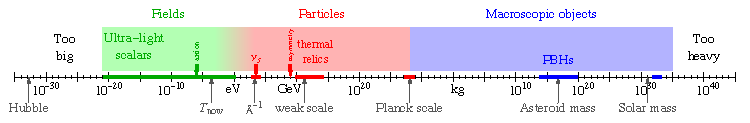
\includegraphics[width=0.95\textwidth]{chapter_01/figures/MDMscale.pdf}
	\caption{The dark-matter mass landscape: viable candidate masses span roughly ninety orders of magnitude, from ultra-light bosonic fields to macroscopic primordial black holes.
		Each class is characterized by a distinct production mechanism and probed by a complementary set of experiments.
		Credit: Cirelli et al.~\cite{Cirelli:2024ssz}. \aure{consider replacing with a custom figure for the final version}}
	\label{fig:dm_mass_landscape}
\end{figure}

Having ruled out every Standard Model particle as the dominant matter component --- \blue{dark matter outweighs baryons by roughly a factor of five} (Section~\ref{sec:1.1.3}), while species that were relativistic at decoupling, such as Standard Model neutrinos, free-stream out of the forming potential wells that observations require~\cite{Bullock:2017xww} --- the search turns to new physics.
As Figure~\ref{fig:dm_mass_landscape} illustrates, the range of possibilities is enormous: 
from ultra-light bosonic fields near $10^{-22}$~eV, below which the de~Broglie wavelength would exceed the size of observed dwarf galaxies~\cite{Hu:2000ke}, up to macroscopic primordial black holes of tens of solar masses, and interaction strengths range from purely gravitational to just below current direct-detection sensitivity.
A separate, quantum-mechanical floor on fermionic candidates comes from the \emph{Tremaine--Gunn bound}~\cite{Tremaine:1979we,Boyarsky:2018tvu}: Pauli exclusion limits the phase-space density that a fermionic species can achieve, requiring $m \gtrsim 0.4$--$1$~keV to match the inner profiles observed in dwarf-spheroidal halos.
\blue{Dark matter must therefore be a new, non-baryonic particle: either \emph{cold} (non-relativistic at decoupling, negligible free-streaming length) or at most \emph{warm} (semi-relativistic, free-streaming length intermediate between neutrino-like relics and cold candidates, suppressing small-scale structure without erasing it).}
The open question is which microphysical realization Nature has chosen.

\Glspl{WIMP_} constitute one of the most popular cold dark matter candidates. They have masses in the GeV--TeV range and interact with Standard Model particles through weak-scale couplings.
They are produced through thermal freeze-out in the early Universe, a mechanism we describe in detail in Section~\ref{sec:1.2.2}.
% The observation that a particle with weak-scale mass and coupling naturally yields the observed relic abundance --- the \WIMP miracle --- has made \glspl{WIMP_} one of the dominant paradigms in the dark matter field for over two decades.
\blue{The \emph{\WIMP miracle} (Section~\ref{sec:1.2.2}) has kept them among the dominant paradigms in the field so far.}
% Concrete realizations include the lightest neutralino of supersymmetric extensions of the Standard Model~\cite{Ellis:1983ew} and \emph{minimal dark matter} scenarios in which a single electroweak multiplet, stabilized by an accidental symmetry, yields the correct relic density without additional model building~\cite{Cirelli:2005uq}.
Concrete realizations include the lightest neutralino of supersymmetric extensions of the Standard Model~\cite{Ellis:1983ew} and \emph{minimal dark matter} scenarios~\cite{Cirelli:2005uq}.
% The same annihilation cross section that sets the relic density also fixes the rate at which \glspl{WIMP_} annihilate into gamma rays in present-day halos, so that indirect-detection signals provide a complementary probe to cosmological measurements of the relic abundance.
% (cut: duplicate of the single-quantity statement at the close of \S\ref{sec:1.2.1} and of \S\ref{sec:1.2.2})
% probe directly the parameter that cosmology constrains.

% Axions are among the most popular alternatives to \glspl{WIMP_}, and as direct-detection limits on \glspl{WIMP_} have tightened, they have drawn growing attention from the dark matter community.
% The axion was originally proposed by Peccei and Quinn~\cite{Peccei:1977hh} as the pseudo-Nambu--Goldstone boson of a spontaneously broken global symmetry introduced to solve the strong CP problem of QCD~\cite{Weinberg:1977ma,Wilczek:1977pj}.
\blue{Axions are among the most popular alternatives to \glspl{WIMP_}, and as direct-detection limits on \glspl{WIMP_} have tightened, they have drawn growing attention from the dark matter community.
The axion was originally proposed by Peccei and Quinn~\cite{Peccei:1977hh} to solve the strong CP problem of QCD~\cite{Weinberg:1977ma,Wilczek:1977pj}.}
It acquires a small mass at the QCD phase transition, and an initial misalignment between its field value and the potential minimum sources a coherent oscillating condensate that today behaves as cold dark matter~\cite{Preskill:1982cy,Abbott:1982af,Dine:1982ah}.
% This \emph{misalignment mechanism}~\cite{Preskill:1982cy,Abbott:1982af,Dine:1982ah} is generic to any light scalar with a late-developing potential and naturally explains why such a feebly coupled particle can saturate the observed relic density.
% Because axions are bosons, they evade the Tremaine--Gunn bound and can sit at occupation numbers $N \gg 1$, behaving as a classical field rather than as a gas of quanta.
\blue{Because axions are bosons, they evade the Tremaine--Gunn bound and can behave as a classical field.}
The phenomenologically viable range of axion masses is broad, spanning roughly $10^{-12}$ to $10^{7}$~eV once astrophysical, cosmological, and laboratory bounds are combined~\cite{Adams:2022pbo, ciaran_o_hare_2020_3932430}.
% Haloscope experiments such as ADMX search for the resonant conversion of the local axion field into microwave photons inside a tunable cavity threaded by a strong magnetic field; the Snowmass community white paper documents the breadth of the dedicated experimental program~\cite{Adams:2022pbo}.


A separate keV-scale window is occupied by sterile (right-handed) neutrinos, which do not couple to the Standard Model weak interaction but mix with active neutrinos.
Two production mechanisms are commonly considered: the Dodelson--Widrow scenario of non-resonant oscillations in the early Universe~\cite{Dodelson:1993je}, and the Shi--Fuller mechanism in which a primordial lepton asymmetry drives resonant oscillations and shifts the produced spectrum to colder momenta~\cite{Shi:1998km}.
Resonant production is the more flexible of the two because it evades the most stringent free-streaming bounds from Lyman-$\alpha$ forest data and Milky Way satellite counts, which otherwise push the allowed mass above $20$--$30$~keV~\cite{Boyarsky:2018tvu}.
Sterile neutrinos are quasi-stable but decay radiatively as $N \to \nu\gamma$, yielding a monochromatic X-ray line that provides a distinctive observational signature~\cite{Boyarsky:2018tvu,Drewes:2016upu}.


%%%%%%%%%%%%

\Glspl{PBH_} offer a qualitatively different option in which the dark matter is not a new particle at all, but a population of macroscopic objects formed from the collapse of large density perturbations before \BBN.
Because \glspl{PBH_} are not made of baryons after \BBN, they bypass the baryon-budget constraint of Section~\ref{sec:1.1.3}.
Microlensing surveys, dynamical bounds on wide stellar binaries and ultra-faint dwarfs, and \CMB spectral-distortion limits together exclude \glspl{PBH_} as the dominant dark-matter component across most of the mass range~\cite{Carr:2020xqk, bradley_j_kavanagh_2019_3538999}.
The single surviving window for a monochromatic \PBH population to constitute all of the dark matter is the asteroid-mass range, $10^{-16}\,M_\odot \lesssim M \lesssim 3 \times 10^{-12}\,M_\odot$, where Hawking-evaporation bounds from below and microlensing limits from above leave a narrow gap that next-generation experiments aim to close. 

An alternative production mechanism is \emph{freeze-in}, in which \glspl{FIMP_} couple so weakly to the thermal bath that they never reach equilibrium~\cite{Hall:2009bx}.
Their abundance is built up gradually through processes like rare decays and $2 \to 2$ scatterings, and the final relic density grows with the coupling rather than shrinking --- the inverse of the freeze-out logic described in Section~\ref{sec:1.2.2}.
% The viable \FIMP mass range is broad, and the extreme smallness of the couplings would make \glspl{FIMP_} difficult to probe in direct-detection experiments or through direct production at colliders, shifting much of the emphasis to cosmological and astrophysical signatures.

Beyond these candidate-based classifications, dark matter may also depart from the cold, collisionless scenario on which $\Lambda$CDM is built.
Several persistent tensions at sub-galactic scales motivate this possibility: the cusp/core problem in dwarf galaxies~\cite{Flores:1994gz,Moore:1994yx}, the diversity of rotation curves at fixed maximum circular velocity~\cite{Oman:2015xda}, and the too-big-to-fail puzzle of the Milky Way satellites~\cite{Boylan-Kolchin:2011qkt,Boylan-Kolchin:2011lmk} all point to fewer dense, cuspy halos than collisionless $N$-body simulations predict~\cite{Bullock:2017xww}.
One alternative is \emph{\WDM}, a kinematic classification encompassing any candidate with a free-streaming length intermediate between hot and cold relics; the resulting suppression of small-scale power softens these tensions while leaving the large-scale successes of $\Lambda$CDM intact.
Resonantly produced keV sterile neutrinos are one concrete realization, but \WDM as a classification is broader, and the astrophysical tests that constrain it are reviewed in~\cite{Adhikari:2022sbh}.
A second, orthogonal direction is \emph{self-interacting dark matter} (SIDM), originally proposed by Spergel and Steinhardt~\cite{Spergel:1999mh} to thermalize the inner regions of halos through elastic scattering and so produce cored rather than cuspy density profiles.
% The relevant figure of merit is the cross section per unit mass: values of order $\sigma/M \sim 1~\mathrm{cm}^2/\mathrm{g}$ at dwarf-galaxy velocities produce a noticeable astrophysical effect, while bullet-cluster and cluster-scale observations require $\sigma/M \lesssim 1~\mathrm{cm}^2/\mathrm{g}$ globally and $\lesssim 0.1~\mathrm{cm}^2/\mathrm{g}$ at cluster velocities, motivating velocity-dependent SIDM models with a light mediator~\cite{Kaplinghat:2015aga}.
The review of Tulin and Yu~\cite{Tulin:2017ara} summarizes the status of the program, and the ETHOS framework~\cite{Cyr-Racine:2015ihg} provides a systematic way to integrate non-standard dark-matter interactions into cosmological hydrodynamical simulations for direct comparison with dwarf-galaxy data.

These examples of candidates make clear how little the existing evidence constrains the microphysics of the dark sector.
We narrow our attention now to the \WIMP paradigm --- the candidate class probed by the gamma-ray indirect-detection analyses developed in the later chapters of this thesis.
The appeal of this framework is that its phenomenology is governed by a single quantity, the velocity-averaged annihilation cross section $\langle\sigma v\rangle$, which simultaneously fixes the cosmological relic abundance, the elastic-scattering rate on nuclei, the production cross section at colliders, and \blue{--- under some assumptions ---} the present-day annihilation rate in galactic halos.
The following subsection reviews the freeze-out mechanism that explains how $\langle\sigma v\rangle$ governs the relic density, and why it defines a natural benchmark for the experimental program that follows.


% The following subsection develops the thermal freeze-out picture quantitatively and shows why the resulting target value of $\langle\sigma v\rangle$ is the natural benchmark of the experimental program that follows.

\subsection{The Freeze-Out Mechanism}
\label{sec:1.2.2}

Consider a hypothetical species $\chi$ held in chemical equilibrium with the Standard Model plasma of the early Universe, sustained by pair-annihilation reactions $\chi\chi \leftrightarrow \mathrm{SM}\,\mathrm{SM}$ that proceed in both directions at equal rates.
As the Universe expands and cools, two processes run in competition: the cosmological expansion, which dilutes everything and lowers the temperature, and the annihilation rate, which depends on the density of $\chi$ particles still available to find each other.
Eventually the expansion wins: the reactions become too slow to maintain equilibrium, the comoving number density stops tracking its equilibrium value, and whatever population remains is locked in as the relic abundance we observe today.
\blue{The purpose of this subsection is to identify what kind of particle reproduces $\Omega_\chi h^2 \approx 0.12$, and to show that the main quantity that controls the process is the velocity-averaged annihilation cross section $\sigmav$.}

A particle that annihilates strongly enough stays in chemical equilibrium for a long time (blue curve in Figure~\ref{fig:freezeout_yx}): it follows the equilibrium population as the latter drops exponentially, and only departs from it when the equilibrium abundance has already become small.
Such a particle leaves behind few relics.
A particle that annihilates weakly (red curve), by contrast, loses contact with the bath earlier, while its equilibrium abundance is still relatively large, and therefore freezes out at a higher residual density.
In the thermal-relic context, the weakest particle wins.
\blue{The relic abundance is thus set to first approximation by how little a candidate annihilates --- by the velocity-averaged annihilation rate $\langle \sigma v_\mathrm{rel}\rangle$ --- while the mass enters only at second order, logarithmically, through the temperature at which decoupling occurs.}

\begin{figure}[t]
	\centering
	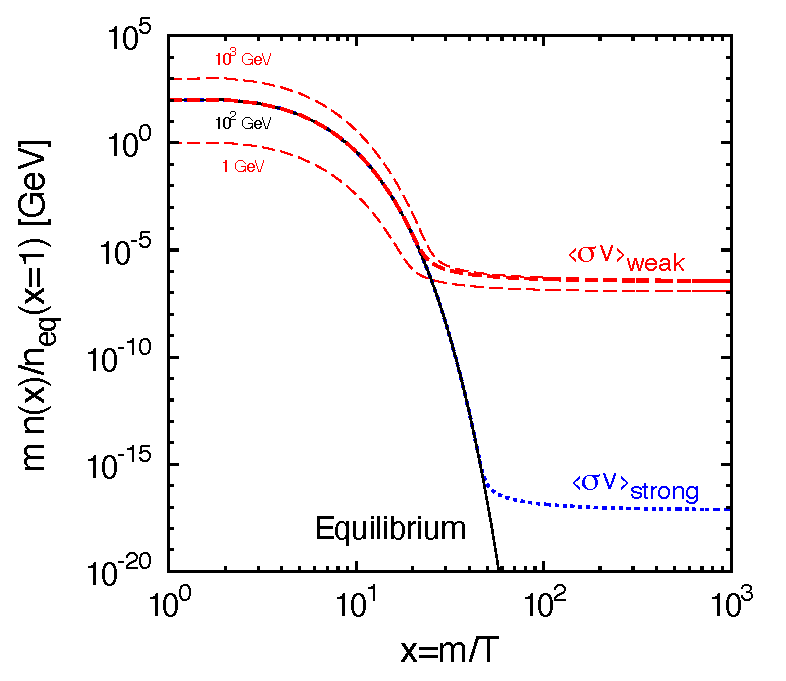
\includegraphics[width=0.7\textwidth]{chapter_01/figures/Steigman2012nb_fig1_v2.pdf}
	\caption{Freeze-out of a thermal relic as a function of the dimensionless inverse temperature $x \equiv M_\chi/T$.
		\blue{The vertical axis is $M_\chi\, n(x)/n_\mathrm{eq}(x{=}1)$ (in GeV), i.e.\ the mass times the comoving number density normalised to the equilibrium value at $x=1$. Up to a constant this is proportional to $M_\chi Y$, with $Y \equiv n_\chi/s$ the comoving abundance, so that the post--freeze-out plateau measures the relic \emph{mass} density directly and hence $\Omega_\chi h^2$.
		The solid black curve traces the equilibrium abundance, exponentially Boltzmann-suppressed once $T$ falls below $M_\chi$ ($x \gtrsim 1$): while annihilations remain faster than the Hubble rate the abundance tracks equilibrium, and once they become inefficient it freezes out at a constant comoving value.
		The thick red (dashed) curve corresponds to a weak-scale cross section $\langle\sigma v\rangle_\mathrm{weak}$, shown as a band for WIMP masses of $1$, $10^2$ and $10^3$~GeV to illustrate the near mass-independence of the freeze-out, while the blue (dotted) curve shows a much larger $\langle\sigma v\rangle_\mathrm{strong}$: a stronger annihilation cross section tracks equilibrium longer and freezes out at a smaller residual abundance ($Y_\infty \propto 1/\langle\sigma v\rangle$).
		Credit: Steigman et al.~\cite{Steigman:2012nb}.}}
	\label{fig:freezeout_yx}
\end{figure}

\blue{Coming back to Figure~\ref{fig:freezeout_yx}, its vertical axis tracks} the comoving abundance $Y \equiv n_\chi/s$ \blue{(up to a mass factor $M_\chi$; see caption)} against the dimensionless inverse temperature $x \equiv M_\chi/T$.
\blue{Here $s = (2\pi^2/45)\, g_{*s}\, T^3$ is the entropy density of the thermal bath; since the comoving entropy $s\,a^3$ is conserved under adiabatic expansion, dividing $n_\chi$ by $s$ factors out the dilution due to the expanding volume, so that a constant $Y$ signals a conserved number of particles per comoving volume.}
At high temperatures ($x \ll 1$), $\chi$ is effectively relativistic and present in numbers comparable to the photons; the actual abundance follows the equilibrium curve $Y_\mathrm{eq}$.
Once the temperature drops below the rest mass ($x \gtrsim 1$), producing a $\chi$ pair costs an exponential Boltzmann penalty, and $Y_\mathrm{eq}$ falls off as $e^{-x}$.
The actual abundance tracks this decline only as long as the annihilation rate $\Gamma = n_\chi \langle \sigma v_\mathrm{rel}\rangle$ exceeds the Hubble rate $H$; once $\Gamma$ drops below $H$, annihilations can no longer keep up with expansion, $Y$ moves away from $Y_\mathrm{eq}$, and the comoving abundance plateaus at its asymptotic value $Y_\infty$.
\blue{This departure is gradual: the dark-matter abundance begins to move away from the equilibrium curve around $x \sim 10$--$15$, while the plasma is still at a temperature of order a tenth of $M_\chi$, and only settles onto its frozen plateau somewhat later.
For a weakly interacting candidate at the electroweak scale, the \emph{freeze-out} completes at $T_\mathrm{fo} \sim M_\chi/(20\text{--}25)$ --- when the particles are already non-relativistic, but the Universe is still deep in radiation domination.}

A quantitative description of this process follows the comoving number density through a variation of the Boltzmann equation \blue{--- here in the reduced, number-density form}~\cite{Gondolo:1990dk,Cirelli:2024ssz},\footnote{\blue{Equation~\eqref{eq:boltzmann} rests on several simplifying assumptions~\cite{Gondolo:1990dk,Cirelli:2024ssz}. The Universe is treated as homogeneous --- primordial inhomogeneities are of order $10^{-5}$, so the number density carries no appreciable spatial dependence. Rapid elastic scattering off the thermal bath keeps the dark matter in kinetic equilibrium: its momentum distribution stays thermal, a single equation for the integrated density $n_\chi(t)$ suffices, and $\langle \sigma v_\mathrm{rel}\rangle$ is averaged over that distribution. The occupation numbers are Maxwell--Boltzmann, appropriate in the non-relativistic regime, and no particle--antiparticle asymmetry is present. Finally, a single species dominates, with $2\to 2$ annihilation as the only relevant process (co-annihilations are deferred to Section~\ref{sec:1.2.4}), and detailed balance fixes the creation term to $\langle \sigma v_\mathrm{rel}\rangle\, n_\mathrm{eq}^2$.}}
\begin{equation}
	\dot n_\chi + 3 H n_\chi = -\langle \sigma v_\mathrm{rel} \rangle\, \bigl( n_\chi^2 - n_\mathrm{eq}^2 \bigr)\,,
	\label{eq:boltzmann}
\end{equation}
where $H$ is the Hubble expansion rate, $n_\mathrm{eq}$ the equilibrium number density, and $n_\chi$ the dark matter number density.
$3 H n_\chi$ is the dilution due to Hubble expansion;  $-\langle \sigma v_\mathrm{rel}\rangle\, n_\chi^2$ is the depletion of $\chi$ by annihilation into Standard Model final states; and $+\langle \sigma v_\mathrm{rel}\rangle\, n_\mathrm{eq}^2$ is the inverse process, in which $\chi$ pairs are recreated from the thermal bath at the rate dictated by detailed balance.
\blue{The expansion rate $H$ is itself fixed by the Friedmann equation, which ties it to the total energy density of the Universe; during the radiation-dominated era that density is set by the relativistic species of the plasma, $\rho \propto g_*\, T^4$ --- with $g_*$ the effective number of relativistic degrees of freedom --- so that $H \sim T^2/M_\mathrm{Pl}$.
Chemical equilibrium persists only as long as the annihilation rate $\Gamma$ remains above this value.}
It is convenient to factor out the trivial expansion dilution by passing from $n_\chi$ to the \emph{comoving abundance} $Y \equiv n_\chi / s$, where $s$ is the entropy density.
Because the total entropy in a comoving volume is conserved during adiabatic expansion, $Y$ remains constant whenever the dark-matter number per comoving volume is also conserved; variations of $Y$ thus track only annihilation and creation, rather than the cosmological dilution shared by every species.
\blue{After freeze-out both annihilation and creation become negligible, and $Y$ approaches a constant value $Y_\infty$; the present-day mass density in dark matter is then $\rho_\chi = M_\chi\, s_0\, Y_\infty$, with $s_0$ the entropy density today.
Dividing by the critical density gives the relic abundance
\begin{equation}
	\Omega_\chi = \frac{M_\chi\, s_0\, Y_\infty}{\rho_\mathrm{crit}}\,, \qquad \rho_\mathrm{crit} = \frac{3 H_0^2}{8\pi G}\,,
	\label{eq:omega_Y}
\end{equation}
which, evaluated with the measured entropy density and expansion rate, can be recast numerically as $Y_\infty \simeq (0.44~\mathrm{eV}/M_\chi)\,(\Omega_\chi h^2/0.12)$.
The observed abundance therefore fixes the product $M_\chi\, Y_\infty$: a heavier candidate must survive in smaller numbers to supply the same mass density.}

A subtlety worth flagging is the meaning of $\langle \sigma v_\mathrm{rel}\rangle$, since the dark-matter literature uses the term ``cross section'' for two physically distinct objects.
The $\sigma v_\mathrm{rel}$ that enters Eq.~\eqref{eq:boltzmann} (in units of cm$^3$/s) is the cross section for the process $\chi\chi \to \mathrm{SM}\,\mathrm{SM}$ multiplied by the relative velocity of the incoming pair, then averaged over a Maxwell--Boltzmann distribution at temperature $T$.
The cross section quoted in direct-detection experiments (in units of cm$^2$), by contrast, is the elastic cross section $\sigma_{\chi N}$ for the recoil process $\chi + N \to \chi + N$ on a target nucleon, involving no thermal average.
The two thus refer to different reactions, different kinematics, and different epochs in the dark-matter history.
Throughout this thesis the symbol $\langle \sigma v\rangle$ always denotes the annihilation case.
% One further point is that the relevant velocity averaging is performed at $T \sim M_\chi/25$ for freeze-out, but at $v \sim 10^{-3} c$ for indirect detection in present-day galactic halos; this mismatch motivates the velocity-dependent cases discussed in Section~\ref{sec:1.2.4}.
One further subtlety is that the thermal average entering the Boltzmann equation is evaluated at freeze-out velocities \blue{of order the thermal scale, $v_\mathrm{rel} \sim \sqrt{T_\mathrm{fo}/M_\chi} \approx 0.2\,c$}, whereas dark-matter particles in present-day galactic halos move at velocities set by the gravitational potential, $v_\mathrm{rel} \sim 10^{-3}\,c$ --- roughly two orders of magnitude smaller.
Whether $\langle \sigma v \rangle$ depends on the relative velocity therefore controls the mapping between the cosmological cross section that fixes the relic abundance and the annihilation rate accessible to indirect detection.
\blue{To keep track of this dependence we expand the annihilation rate in partial waves, and defer its observational consequences to Section~\ref{sec:1.2.4}.}

Non-relativistic two-body annihilation admits the partial-wave expansion
\begin{equation}
	\sigma v_\mathrm{rel} \simeq \sigma_0 + \sigma_1\, v_\mathrm{rel}^2 + \mathcal{O}(v_\mathrm{rel}^4)\,,
	\label{eq:partial_wave}
\end{equation}
where $\sigma_0$ is the $s$-wave ($\ell=0$) contribution and $\sigma_1\, v_\mathrm{rel}^2$ the $p$-wave ($\ell=1$) contribution~\cite{Cirelli:2024ssz}.
\blue{Averaging this expansion over the thermal distribution of relative velocities gives $\langle \sigma v_\mathrm{rel}\rangle = \sigma_0 + (6T/M_\chi)\,\sigma_1 + \cdots$; at freeze-out, with $x_\mathrm{fo} \equiv M_\chi/T_\mathrm{fo}$, the $p$-wave term is therefore suppressed by a factor $6/x_\mathrm{fo}$ relative to the $s$-wave piece.}

\blue{Solving Eq.~\eqref{eq:boltzmann} through the freeze-out transition places the decoupling at $x_\mathrm{fo} \approx 25$, consistent with the value $T_\mathrm{fo} \sim M_\chi/(20\text{--}25)$ anticipated above; this number depends only logarithmically on the dark-matter mass and couplings, so candidates spanning a broad range of masses freeze out at comparable $x$.
The surviving comoving abundance then scales as
\[
	Y_\infty \propto \frac{x_\mathrm{fo}}{M_\mathrm{Pl}\, M_\chi\, (\sigma_0 + 3\sigma_1/x_\mathrm{fo})}\,,
\]
inversely proportional to the annihilation strength; the $p$-wave coefficient enters here as $3\sigma_1/x_\mathrm{fo}$ --- rather than the $6\sigma_1/x_\mathrm{fo}$ of the instantaneous thermal average --- because annihilations continue to deplete the abundance after freeze-out, so the velocity-dependent term is averaged over the subsequent evolution rather than sampled at $T_\mathrm{fo}$ alone.
Inserting this into Eq.~\eqref{eq:omega_Y} yields the relic density in terms of the partial-wave coefficients~\cite{Steigman:2012nb,Cirelli:2024ssz},
\begin{equation}
	\frac{\Omega_\chi h^2}{0.12} \approx \frac{x_\mathrm{fo}}{25}\,\frac{2.2\times 10^{-26}~\mathrm{cm^3/s}}{\sigma_0 + 3\sigma_1/x_\mathrm{fo}}\,.
	\label{eq:relic_general}
\end{equation}
In the limit of pure $s$-wave annihilation the coefficient $\sigma_1$ vanishes, the thermal average becomes the constant $\langle \sigma v_\mathrm{rel}\rangle = \sigma_0$, and Eq.~\eqref{eq:relic_general} reduces, for $x_\mathrm{fo}\approx 25$, to}
\begin{equation}
	\frac{\Omega_\chi h^2}{0.12} \approx \frac{2.2 \times 10^{-26}~\mathrm{cm^3/s}}{\langle \sigma v_\mathrm{rel}\rangle}\,,
	\label{eq:relic_abundance}
\end{equation}
where the relic abundance is essentially the inverse of the annihilation cross section, with the mass entering only through logarithmic corrections to the prefactor.
The numerator is the canonical \emph{thermal cross section}, $\langle \sigma v\rangle_\mathrm{cosmo} \approx 2.2 \times 10^{-26}$~cm$^3$/s: any dark-matter candidate that annihilates at this rate reproduces, \blue{to within a few percent for masses above roughly $10$~GeV (cf.~Figure~\ref{fig:thermal_relic})}, the observed cosmological abundance.
For an annihilation amplitude characterized by a coupling $g$, with $\alpha \equiv g^2/(4\pi)$, the natural size of the cross section is $\langle \sigma v\rangle \sim \alpha^2/M_\chi^2$.
Plugging in the weak-interaction value $\alpha \sim \alpha_\mathrm{weak} \sim 0.03$ and demanding a match to $\langle \sigma v\rangle_\mathrm{cosmo}$ returns a mass $M_\chi$ of order a few hundred GeV to a few TeV --- the electroweak scale.
% , recovered without any input from particle-physics model-building.
This result is known as the \emph{\WIMP miracle}: a stable particle with mass and coupling strength at the electroweak scale, produced thermally in the early Universe, naturally yields a relic abundance consistent with the observed dark matter density~\cite{Cirelli:2024ssz,Steigman:2012nb}.
\blue{The inverse relation of Eq.~\eqref{eq:relic_abundance} is illustrated in Figure~\ref{fig:thermal_relic}: the orange band marks the cross section that reproduces the measured abundance, while smaller (larger) values freeze out too early (too late) and overproduce (underproduce) dark matter.}

\begin{figure}[t]
	\centering
	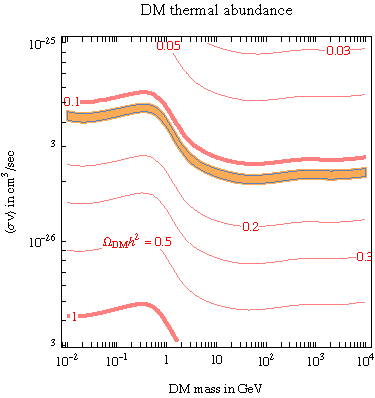
\includegraphics[width=0.47\textwidth]{chapter_01/figures/Omegafreeze-out.pdf}
	\caption{Contours for the dark matter freeze-out abundance $\Omega_\text{DM} h^2$ as a function of DM mass and annihilation cross-section $\langle \sigma v \rangle$ for Majorana dark matter.
	The measured cosmological abundance $\Omega_\text{DM} h^2 = 0.120 \pm 0.001$ is reproduced within the orange band at $3\sigma$.
	From this plot it is possible to appreciate how the annihilation cross-section needed to match the observed abundance varies with mass in the $1-3 \times 10^{-26} \, \textrm{cm}^3/\textrm{s}$ range.
	Credit: Cirelli et al.~\cite{Cirelli:2024ssz}.
	}
	\label{fig:thermal_relic}
\end{figure}

In the same $s$-wave limit, the cross section fixed by Eq.~\eqref{eq:relic_abundance} also sets the rate at which dark matter annihilates in present-day astrophysical environments.
This connection between cosmological abundance and indirect-detection signals further motivates the gamma-ray searches of Chapters~\ref{ch:4}--\ref{ch:8}.

\subsection{Theoretical Bounds on the WIMP Mass}
\label{sec:1.2.3}

% The relic-abundance formula of the previous subsection, combined with some additional physical requirements, brackets the viable \WIMP mass from both below and above.
%
In this section we explore the viable mass range for \glspl{WIMP_}.
Consider first a particle that interacts with the Standard Model only through the weak interaction, with no dark mediator of its own.
At freeze-out energies, using the Fermi approximation, the annihilation cross section for such a particle, dominated by exchange of $W$ and $Z$ bosons, scales as $\sigma_0 \approx G_F^2 M_\chi^2 / 2\pi$, where $G_F$ is the Fermi constant~\cite{Bertone:2004pz}.
This is an \emph{$s$-wave} process \blue{(cf.~Eq.~\eqref{eq:partial_wave})}, meaning the cross section is independent of the relative velocity --- a noteworthy property, since it distinguishes whether or not the same $\sigmav$ that fixes the relic abundance also drives present-day annihilations in galactic halos.
Because $\sigma_0$ scales as $M_\chi^2$ \blue{in this approximation}, lowering the candidate mass reduces the annihilation cross section quadratically; combined with the inverse dependence of the relic abundance on $\sigmav$ in Eq.~\eqref{eq:relic_abundance}, this means a sufficiently light particle annihilates too weakly to thin itself out and ends up overproducing dark matter.
The original Lee--Weinberg analysis~\cite{Lee:1977ua}, contemporaneous with the closely related arguments of Hut~\cite{Hut:1977zn} and Vysotsky, Dolgov, and Zeldovich~\cite{Vysotsky:1977pe}, obtained $M_\chi \gtrsim 2$~GeV for a heavy Dirac neutrino. Modern evaluations with updated effective-degree-of-freedom counts give~\cite{Cirelli:2024ssz,Bertone:2004pz}
\begin{equation}
	M_\chi \gtrsim 3~\mathrm{GeV} \qquad \text{(Lee--Weinberg bound)}\,,
	\label{eq:lee_weinberg}
\end{equation}
below which a thermal relic coupled to the Standard Model weak interaction is cosmologically forbidden.
This GeV-scale floor is specific to annihilation mediated by W and Z bosons. When that assumption is dropped, the much weaker \BBN bound discussed below takes over, extending the allowed lower edge into the MeV regime.

It is important to stress the coupling with the Standard Model weak interaction.
The Lee--Weinberg bound says nothing about models in which a new mediator --- a dark photon, a light scalar, or a hidden-sector gauge boson --- carries the annihilation.
With such ingredients the relic abundance can be reproduced down to the sub-GeV and even keV regimes, which is precisely why a parallel low-mass direct-detection program (SENSEI, DAMIC, and related semiconductor experiments~\cite{SENSEI:2020dpa,DAMIC-M:2023gxo}) has grown alongside the conventional GeV--TeV searches.

The upper end of the mass window has a more universal origin, which is often referred to as the \emph{unitarity bound}.
Quantum mechanics requires probabilities to sum to one; in scattering theory this \emph{unitarity} condition bounds the cross section for any two-body process from above by a quantity set purely by the available phase space, $\sigma \leq 4\pi/k^2$, where $k = M_\chi v/2$ is the center-of-mass momentum~\cite{Griest:1989wd}.
For non-relativistic dark-matter annihilation this translates directly to $\langle \sigma v \rangle_\mathrm{max} \propto 1/M_\chi^2$, a ceiling that any model must respect regardless of its coupling structure.
As the candidate mass increases, the unitarity ceiling drops; at some mass it sinks below the thermal benchmark $\langle \sigma v \rangle_\mathrm{cosmo}$, and beyond that point even a maximally coupled candidate must be overabundant.
The classic estimate of Griest and Kamionkowski places this crossover at~\cite{Griest:1989wd}
\begin{equation}
	M_\chi \lesssim 100~\mathrm{TeV}\,, \qquad \text{(unitarity bound)}
	\label{eq:unitarity}
\end{equation}
above which thermal-relic dark matter is no longer viable as a single-particle, two-body annihilation problem and requires either bound-state formation, multi-step annihilation cascades, or a non-thermal cosmological history.

% A closely related but logically distinct constraint comes from \emph{perturbativity}.
% A renormalizable model with dimensionless coupling $g$ admits a controlled perturbative expansion only as long as $g^2 \lesssim 4\pi$; beyond that point, loop corrections compete with tree-level amplitudes and the calculation loses its meaning even if the theory remains nominally consistent.
% Because $\langle \sigma v \rangle \sim g^4 / M_\chi^2$ for a generic $2\to 2$ annihilation, perturbativity caps the achievable cross section at a value that, like the unitarity ceiling, falls with mass.
% The distinction between the two is conceptually instructive: perturbativity is a \emph{theory-quality} constraint that says we no longer trust our calculation, while unitarity is a \emph{physics-quality} constraint that says no physical theory can do better; the unitarity bound is the conservative one generally adopt.

An independent lower bound, insensitive to which mediator carries the annihilation, comes from \BBN~\cite{Nollett:2014lwa}.
A dark-matter particle still in chemical contact with the plasma at $T \sim 1$~MeV would contribute to the radiation energy density during nucleosynthesis and inject electromagnetic or hadronic energy through residual annihilations, both of which spoil the otherwise excellent agreement between predicted and observed primordial light-element abundances.
Requiring freeze-out to complete before \BBN enforces $M_\chi \gtrsim 3$~MeV, a floor that holds for any thermal relic regardless of its couplings.

Taken together, these arguments delineate a mass window
\begin{equation}
	3~\mathrm{GeV} \lesssim M_\chi \lesssim 100~\mathrm{TeV}\,,
	\label{eq:wimp_window}
\end{equation}
for \glspl{WIMP_} that annihilate through Standard Model weak interactions, with the \BBN floor extending the lower edge into the MeV regime for candidates with non-Standard-Model mediators.
Within this window the thermal benchmark $\langle \sigma v \rangle_\mathrm{cosmo} \approx 2.2 \times 10^{-26}~\mathrm{cm}^3/\mathrm{s}$ is the natural target for indirect-detection experiments: any instrument that reaches this sensitivity directly tests the thermal freeze-out hypothesis.
The Fermi Large Area Telescope already reaches the benchmark in the $b\bar b$ channel up to masses of several tens of GeV looking at \glspl{dSph_}, an analysis we revisit in \blue{Chapter~\ref{ch:5}} when studying dark matter subhalos. The Cherenkov Telescope Array Observatory, with its larger collection area and lower energy threshold relative to current imaging atmospheric Cherenkov arrays, will extend indirect-detection sensitivity into the TeV domain, which is the subject of Chapter~\ref{ch:8}.
% We close with a caveat: the bounds derived here assume the simplest freeze-out scenario --- a single stable species annihilating through a velocity-independent $s$-wave amplitude --- and several physically motivated effects can shift the mapping between $\langle \sigma v \rangle_\mathrm{cosmo}$ and the present-day indirect-detection signal in either direction. We briefly survey alternative freeze-out scenarios in the next subsection.

\subsection{\blue{Beyond s-wave annihilation}}
\label{sec:1.2.4}

The bounds derived in Section~\ref{sec:1.2.3} assumed the simplest possible freeze-out scenario: a single stable species, \blue{$s$-wave--dominated two-body annihilation}, and weak-scale couplings.
Several physically motivated effects modify this picture and, more importantly, alter the mapping between the cosmological cross section $\langle\sigma v\rangle_\mathrm{cosmo}$ that fixes the relic abundance and the present-day annihilation rate probed by indirect detection.

\paragraph{$p$-wave suppression.}
\blue{The starting point is the partial-wave expansion of Eq.~\eqref{eq:partial_wave} from Section~\ref{sec:1.2.2}.}
When the $s$-wave piece is \blue{dominant}, the cross section is approximately constant from freeze-out velocities ($v_\mathrm{rel}\sim \blue{0.2}\,c$) down to typical halo velocities ($v_\mathrm{rel}\sim 10^{-3}\,c$), and $\langle\sigma v\rangle_\mathrm{cosmo}$ remains a meaningful benchmark for indirect-detection searches.
When the leading contribution is $p$-wave, in contrast, the present-day rate is suppressed by $v_\mathrm{rel}^2 \sim 10^{-6}$ relative to its value at freeze-out, and the channel becomes effectively invisible to instruments that rely on annihilation in cold galactic halos.
% Selection rules --- for instance, specific initial-state quantum numbers or symmetries of the underlying interaction --- can cause the $s$-wave amplitude to vanish identically in particular models, leaving $p$-wave as the leading contribution and rendering the channel undetectable with gamma-ray telescopes.

\paragraph{Sommerfeld enhancement.}
A second class of corrections arises when dark matter couples to a mediator with mass $M_V \ll M_\chi$.
The long-range attractive force distorts the incoming-pair wave function and enhances the annihilation probability at low velocities, a non-perturbative effect known as the \emph{Sommerfeld enhancement}~\cite{Hisano:2004ds,ArkaniHamed:2008qn}.
\blue{The enhancement factor $S$ grows as the relative velocity falls, roughly as $S\propto 1/v_\mathrm{rel}$, and can be resonantly amplified for particular mediator-to-dark-matter mass ratios.
Halo velocities $v_\mathrm{rel}\sim 10^{-3}\,c$ therefore probe a regime in which $S$ can reach $\mathcal{O}(10^2\text{--}10^3)$~\cite{Hisano:2004ds}, while at freeze-out velocities $v_\mathrm{rel}\sim 0.2\,c$ the enhancement is only moderate.}
The Sommerfeld effect is essential for heavy electroweak \glspl{WIMP_} --- the pure wino at $M_\chi\sim 3\,\mathrm{TeV}$, the higgsino near $M_\chi\sim 1.1\,\mathrm{TeV}$, and Minimal Dark Matter candidates more generally --- where it shifts the thermal-relic mass from hundreds of GeV to multi-TeV scales. We return to this point in Section~\ref{sec:1.4} when discussing $J$-factors and the loop-suppressed channels of Minimal Dark Matter.
For the pure wino in particular, the enhanced halo rate at $v_\mathrm{rel}\sim 10^{-3}\,c$ is large enough that current gamma-ray constraints effectively rule the candidate out for cuspy halo profiles.
For the GeV-scale candidates relevant to the Galactic Center excess analyzed in Chapter~\ref{ch:4}, by contrast, the standard thermal cross section fits the observed signal without invoking Sommerfeld enhancement, as Daylan et al.~\cite{Daylan:2014rsa} showed explicitly for a $\sim \blue{36}$--$\blue{51}\,\mathrm{GeV}$ \WIMP annihilating at $\langle\sigma v\rangle \approx (1$--$3)\times 10^{-26}\,\mathrm{cm}^3/\mathrm{s}$.

\paragraph{Co-annihilation and resonance.}
\blue{Two further refinements deserve mention because they directly affect the indirect detection prospects.
The first is \emph{co-annihilation}: if the dark sector contains partner particles nearly degenerate with $\chi$, they stay abundant during freeze-out and help deplete the dark-matter density~\cite{Ellis:1983ew,Griest:1990kh}.
Since these partners later decay into $\chi$, the present-day annihilation cross section of the surviving species can differ substantially from the effective freeze-out value, weakening the link between $\Omega_\chi h^2$ and the indirect-detection signal.
The second is \emph{resonant annihilation}: when dark matter annihilates through an $s$-channel mediator with mass near threshold, $m_\mathrm{med}\approx 2 M_\chi$, the cross section acquires a sharp velocity dependence of Breit--Wigner form~\cite{Griest:1990kh,Gondolo:1990dk}, so the present-day rate may be either enhanced or suppressed relative to freeze-out.
Both effects introduce model dependence into the mapping from $\langle\sigma v\rangle_\mathrm{cosmo}$ to the observable annihilation rate.}

These refinements lead to several distinct theoretical scenarios, of which the standard case --- $s$-wave annihilation --- is the simplest and the least model-dependent.
In that case, the freeze-out cross section also fixes the galactic-halo annihilation rate \blue{(Section~\ref{sec:1.2.2})}, providing the cleanest target for indirect-detection experiments.
In richer scenarios the mapping remains calculable but model-dependent: Sommerfeld enhancement can boost halo rates by orders of magnitude, $p$-wave suppression or off-resonance Breit--Wigner effects can lower them, and co-annihilation can shift the relic-abundance target relative to the halo signal.
Throughout this thesis we adopt the standard thermal-relic value of $\langle\sigma v\rangle$ as the primary benchmark when quoting cross-section bounds, while flagging explicitly the regimes in which these refinements would shift the interpretation.
With this theoretical setting in place, we turn to the experimental strategies for testing the WIMP hypothesis.
